\chapter{Specifikacija programske potpore}
		
	\section{Funkcionalni zahtjevi}

			\noindent \textbf{Dionici:}
			
			\begin{packed_enum}
				\item Naručitelj
				\item Regularni korisnik		
				\item Kartograf
				\item Administrator
		        \item Razvojni tim
				
			\end{packed_enum}
			
			\noindent \textbf{Aktori i njihovi funkcionalni zahtjevi:}
			
			
			\begin{packed_enum}
				\item  \underbar{Neregistrirani/neprijavljeni korisnik (inicijator) može:}
				
				\begin{packed_enum}
					
					\item Registrirati se u sustav za što je potrebno unijeti email adresu, ime, prezime, korisničko ime i lozinku 
					\item Prijaviti se u sustav za što je potrebno unijeti samo korisničko ime i lozinku
					
				\end{packed_enum}
			
				\item  \underbar{Regularni korisnik (inicijator) može:}
				
				\begin{packed_enum}
					
					\item pregledavati osobne podatke
					\item mijenjati osobne podatke
					\item mijenjati postavke privatnosti vlastitog profila
					\item pretraživati druge korisničke profile
					\item objavljivati putovanja
					\item pregledavati vlastite bedževe
					\item dodavati putovanja na wishlistu
					\item objavljivati prijedloge novih lokacija
					\item osvajati bedževe na putovanjima
					
				\end{packed_enum}
				
				\item  \underbar{Kartograf (inicijator) može:}
				
				\begin{packed_enum}
					
					\item definirati nova pravila za bedževe
					
				\end{packed_enum}
				
				\item  \underbar{Administrator (inicijator) može:}
				
				\begin{packed_enum}
					
					\item uklanjati korisnike iz sustava
					\item odobriti ili odbiti prijedloge novih lokacija
					\item unositi nove lokacije, gradove i države
					
				\end{packed_enum}
				
				\item  \underbar{Baza podataka (sudionik):}
				
				\begin{packed_enum}
					
					\item pohranjuje sve podatke o korisnicima i njihovim ovlastima
					\item pohranjuje sve podatke o korisnikovim putovanjima, bedževima i prijateljima
					
				\end{packed_enum}
			\end{packed_enum}
			
			\eject 
			
			
				
			\subsection{Obrasci uporabe}
				
				
				\subsubsection{Opis obrazaca uporabe}

					\noindent \underbar{\textbf{UC1 - "Registracija}}
					\begin{packed_item}
	
						\item \textbf{Glavni sudionik: }Neregistrirani korisnik, regularni korisnik
						\item  \textbf{Cilj:} Stvoriti korisnički račun za pristup sustavu
						\item  \textbf{Sudionici:} Baza podataka
						\item  \textbf{Preduvjet:} -
						\item  \textbf{Opis osnovnog tijeka:}
						
						\item[] \begin{packed_enum}
	
							\item Korisnik odabire opciju za registraciju
							\item Korisnik unosi potrebne korisničke podatke
							\item Korisnik prima obavijest o uspješnoj registraciji
							\item Korisnik se preusmjerava na početnu stranicu

						\end{packed_enum}
						
						\item  \textbf{Opis mogućih odstupanja:}
						
						\item[] \begin{packed_item}
	
							\item[1.a] Odabir već zauzetog korisničkog imena ili email adrese ili unos korisničkog podatka u nedozvoljenom formatu
							\item[] \begin{packed_enum}
								
								\item Sustav obavještava korisnika o neuspjelom upisu i vraća ga na stranicu za registraciju
								\item Korisnik mijenja potrebne podatke te završava unos ili odustaje od registracije
								
							\end{packed_enum}
						\end{packed_item}
					\end{packed_item}
					
					\noindent \underbar{\textbf{UC2 - "Prijava u sustav}}
					\begin{packed_item}
	
						\item \textbf{Glavni sudionik: }Regularni korisnik
						\item  \textbf{Cilj:} Dobiti pristup korisničkom sučelju (početnoj stranici)
						\item  \textbf{Sudionici:} Baza podataka
						\item  \textbf{Preduvjet:} Registracija
						\item  \textbf{Opis osnovnog tijeka:}
						
						\item[] \begin{packed_enum}
	
							\item Korisnik unosi lozinku i korisničko ime
							\item Potvrda o ispravnosti unesenih podataka
							\item Korisnik se preusmjerava na početnu stranicu

						\end{packed_enum}
						
						\item  \textbf{Opis mogućih odstupanja:}
						
						\item[] \begin{packed_item}
	
							\item[2.a] Neispravno korisničko ime/lozinka
							\item[] \begin{packed_enum}
								
								\item Sustav obavještava korisnika o neuspjelom upisu i vraća ga na stranicu za prijavu
								
							\end{packed_enum}
						\end{packed_item}
					\end{packed_item}
				
				    \noindent \underbar{\textbf{UC3 - "Pregled osobnih podataka}}
					\begin{packed_item}
	
						\item \textbf{Glavni sudionik: }Regularni korisnik
						\item  \textbf{Cilj:} Pregledati osobne podatke
						\item  \textbf{Sudionici:} Baza podataka
						\item  \textbf{Preduvjet:} Korisnik je prijavljen
						\item  \textbf{Opis osnovnog tijeka:}
						
						\item[] \begin{packed_enum}
	
							\item Korisnik odabire opciju "Moj profil"
							\item Aplikacija prikazuje osobne podatke korisnika

						\end{packed_enum}
						
					\end{packed_item}
					
					\noindent \underbar{\textbf{UC4 - "Promjena osobnih podataka}}
					\begin{packed_item}
	
						\item \textbf{Glavni sudionik: }Regularni korisnik
						\item  \textbf{Cilj:} Izmijeniti osobne podatke
						\item  \textbf{Sudionici:} Baza podataka
						\item  \textbf{Preduvjet:} Korisnik je prijavljen i nalazi se na stranici "Moj profil"
						\item  \textbf{Opis osnovnog tijeka:}
						
						\item[] \begin{packed_enum}
	    
	                        \item Korisnik odabire "Uredi profil"
							\item Korisnik mijenja svoje osobne podatke
							\item Korisnik sprema ili odbacuje promjene
							\item Baza podataka se ažurira u slučaju spremanja

						\end{packed_enum}
					\end{packed_item}
					
					\noindent \underbar{\textbf{UC5 - "Pregled osvojenih bedževa}}
					\begin{packed_item}
	
						\item \textbf{Glavni sudionik: }Regularni korisnik
						\item  \textbf{Cilj:} Pregledati osvojeni bedževe
						\item  \textbf{Sudionici:} Baza podataka
						\item  \textbf{Preduvjet:} Korisnik je prijavljen
						\item  \textbf{Opis osnovnog tijeka:}
						
						\item[] \begin{packed_enum}
	
							\item Korisnik odabire opciju "Moji bedževi"
							\item Aplikacija prikazuje osvojene bedževe korisnika

						\end{packed_enum}
						
					\end{packed_item}
					
					\noindent \underbar{\textbf{UC6 - "Pregled vlastite wishliste}}
					\begin{packed_item}
	
						\item \textbf{Glavni sudionik: }Regularni korisnik
						\item  \textbf{Cilj:} Pregledati wishlistu
						\item  \textbf{Sudionici:} Baza podataka
						\item  \textbf{Preduvjet:} Korisnik je prijavljen
						\item  \textbf{Opis osnovnog tijeka:}
						
						\item[] \begin{packed_enum}
	
							\item Korisnik odabire opciju "Lista želja"
							\item Aplikacija prikazuje listu želja

						\end{packed_enum}
						
					\end{packed_item}
					
				    \noindent \underbar{\textbf{UC7 - "Pregled vlastitih putovanja}}
					\begin{packed_item}
	
						\item \textbf{Glavni sudionik: }Regularni korisnik
						\item  \textbf{Cilj:} Pregledati vlastita putovanja
						\item  \textbf{Sudionici:} Baza podataka
						\item  \textbf{Preduvjet:} Korisnik je prijavljen
						\item  \textbf{Opis osnovnog tijeka:}
						
						\item[] \begin{packed_enum}
	
							\item Korisnik odabire opciju "Moja putovanja"
							\item Aplikacija prikazuje putovanja korisnika u obliku objava

						\end{packed_enum}
						
					\end{packed_item}
					
					\noindent \underbar{\textbf{UC8 - "Pregled profila drugih korisnika}}
					\begin{packed_item}
	
						\item \textbf{Glavni sudionik: }Regularni korisnik
						\item  \textbf{Cilj:} Pregledati objave drugih korisnika
						\item  \textbf{Sudionici:} Baza podataka
						\item  \textbf{Preduvjet:} Korisnik je prijavljen
						\item  \textbf{Opis osnovnog tijeka:}
						
						\item[] \begin{packed_enum}
	
							\item Korisnik odabire opciju "Društvo"
							\item Korisnik pretražuje korisnika čije profil želi pogledati

						\end{packed_enum}
						
					\end{packed_item}
					
					\noindent \underbar{\textbf{UC9 - "Označavanje putovanja drugog korisnika sa "Sviđa mi se"}}
					\begin{packed_item}
	
						\item \textbf{Glavni sudionik: }Regularni korisnik
						\item  \textbf{Cilj:} Označiti putovanje drugog korisnika sa "Sviđa mi se"
						\item  \textbf{Sudionici:} Baza podataka
						\item  \textbf{Preduvjet:} Korisnik je prijavljen i pregledava račun korisnika čije postavke privatnosti su postavljene na "javno"
						\item  \textbf{Opis osnovnog tijeka:}
						
						\item[] \begin{packed_enum}
	
							\item Korisnik reagira na putovanje
							\item U bazi podataka se ažurira broj oznaka sa "Sviđa mi se"

						\end{packed_enum}
						
					\end{packed_item}
					
					\noindent \underbar{\textbf{UC10 - "Dodavanje stavki na wishlistu"}}
					\begin{packed_item}
	
						\item \textbf{Glavni sudionik: }Regularni korisnik
						\item  \textbf{Cilj:} Dodati željenu stavku (npr. lokaciju) na wishlistu
						\item  \textbf{Sudionici:} Baza podataka
						\item  \textbf{Preduvjet:} Korisnik je prijavljen i nalazi se na "Lista želja" lokaciji u aplikaciji
						\item  \textbf{Opis osnovnog tijeka:}
						
						\item[] \begin{packed_enum}
	
							\item Korisnik odabire opciju "Nova želja"
							\item Korisnik ispunjava formu za dodavanje novih želja
							\item U bazi podataka se ažurira lista želja korisnika s novom željom

						\end{packed_enum}
						
					\end{packed_item}
					
					\noindent \underbar{\textbf{UC11 - "Pregled karte, osvojenih država i pinova"}}
					\begin{packed_item}
	
						\item \textbf{Glavni sudionik: }Regularni korisnik
						\item  \textbf{Cilj:} Prikazati naslovnicu (početnu stranicu) na kojoj se nalazi karta s obojenim državama i pinovima
						\item  \textbf{Sudionici:} Baza podataka
						\item  \textbf{Preduvjet:} Korisnik je prijavljen
						\item  \textbf{Opis osnovnog tijeka:}
						
						\item[] \begin{packed_enum}
	
							\item Korisnik odabire opciju "Naslovnica"
							\item Prikazuje se stranica "Naslovnica" s kartom i pinovima

						\end{packed_enum}
						
					\end{packed_item}
					
					
					\noindent \underbar{\textbf{UC12 - "Izmjena postavki privatnosti"}}
					\begin{packed_item}
	
						\item \textbf{Glavni sudionik: }Regularni korisnik
						\item  \textbf{Cilj:} Promijeniti postavke privatnosti, specifično prikazuju li se i putovanja ili samo bedževi
						\item  \textbf{Sudionici:} Baza podataka
						\item  \textbf{Preduvjet:} Korisnik je prijavljen i nalazi se na stranici "Moj profil"
						\item  \textbf{Opis osnovnog tijeka:}
						
						\item[] \begin{packed_enum}
	
	                        \item Korisnik odabire "Uredi profil"
							\item Korisnik izmjenjuje postavke privatnosti
							\item U bazi podataka se ažuriraju postavke privatnosti korisnika

						\end{packed_enum}
						
					\end{packed_item}
					
					
					\noindent \underbar{\textbf{UC13 - "Objavljivanje putovanja"}}
					\begin{packed_item}
	
						\item \textbf{Glavni sudionik: }Regularni korisnik
						\item  \textbf{Cilj:} Podijeliti putovanje na profilu
						\item  \textbf{Sudionici:} Baza podataka
						\item  \textbf{Preduvjet:} Korisnik je prijavljen i nalazi se na stranici "Moja putovanja"
						\item  \textbf{Opis osnovnog tijeka:}
						
						\item[] \begin{packed_enum}
	                        \item Korisnik odabire opciju "Nova objava"
							\item Korisnik ispunjava formu za dodavanje novog putovanja
							\item Korisnik odabire jednu od postojećih lokacija ili šalje prijedlog za dodavanje nove lokacije 
							\item Korisnik u formi također mora ispuniti polja:
							\begin{packed_item}
							    \item datum posjeta
							    \item vrsta prijevoza do mjesta
							    \item ocjena gužve
							    \item oznaka putuje li samostalno ili u društvu
							    \item recenzija putovanja - ocjena i komentar
							\end{packed_item}
							\item Provjerava se ispunjava li korisnik uvjete za osvajanje bedža
							\item U bazu podataka se sprema putovanje korisnika te je vidljivo na korisnikovom profilu
		

						\end{packed_enum}
						
						\item  \textbf{Opis mogućih odstupanja:}
						
						\item[] \begin{packed_item}
	
							\item[13.a] Korisnik je odlučio poslati prijedlog za dodavanje nove lokacije
							\item[] \begin{packed_enum}
								
								\item Ako administrator odobri korisnikov zahtjev dodat će se nova lokacija u skup postojećih lokacija u bazi podataka
								
							\end{packed_enum}
							
							\item[13.b] Korisnik ispunjava uvjete za osvajanje bedža
							\item[] \begin{packed_enum}
							    \item Korisniku se dodjeljuje bedž
							    \item U bazi podataka se ažurira lista bedževa korisnika
							\end{packed_enum}
							
							\item[13.c] Korisnik ispunjava uvjete za ispunjavanje želje s wishlista
							\item[] \begin{packed_enum}
							    \item Korisniku se dodjeljuje bedž s wishlista
							    \item U bazi podataka se ažurira lista bedževa korisnika
							    \item Uklanja se želja s liste želja
							\end{packed_enum}
							
						\end{packed_item}
						
					\end{packed_item}
					
					\noindent \underbar{\textbf{UC14 - "Pretraživanje lokacija na karti"}}
					\begin{packed_item}
	
						\item \textbf{Glavni sudionik: }Regularni korisnik
						\item  \textbf{Cilj:} Pronaći traženu lokaciju na karti
						\item  \textbf{Sudionici:} Baza podataka
						\item  \textbf{Preduvjet:} Korisnik je prijavljen i nalazi se na stranici "Moj profil"
						\item  \textbf{Opis osnovnog tijeka:}
						
						\item[] \begin{packed_enum}
	
	                        \item Korisnik odabire "Pretraživanje"
							\item Korisnik upisuje lokaciju koju želi pronaći
							\item Prikazuje se tražena lokacija na karti

						\end{packed_enum}
						
						\item  \textbf{Opis mogućih odstupanja:}
						\item[] \begin{packed_item}
	
							\item[14.a] Ne postoji lokacija koju korisnik traži
							\item[] \begin{packed_enum}
								\item Korisniku se ispisuje odgovarajuća poruka da lokacija koju traži nije pronađena
							\end{packed_enum}
						\end{packed_item}
						
					\end{packed_item}
					
					
					\noindent \underbar{\textbf{UC15 - "Izrada novog bedža"}}
					\begin{packed_item}
	
						\item \textbf{Glavni sudionik: }Kartograf
						\item  \textbf{Cilj:} Kreirati novi bedž
						\item  \textbf{Sudionici:} Baza podataka
						\item  \textbf{Preduvjet:} Kartograf je prijavljen
						\item  \textbf{Opis osnovnog tijeka:}
						
						\item[] \begin{packed_enum}
	
	                        \item Kartograf odabire opciju "Bedževi"
	                        \item Kartograf ispunjava formu za dodavanje novih bedževa:
	                        \begin{packed_item}
							    \item ime bedža
							    \item opis bedža
							    \item slika bedža (sami bedž)
							    \item tip bedža
							    \item pravila bedža
							\end{packed_item}
							\item Ako kartograf odabere opciju "Spremi" novi bedž se kreira i ažurira se lista bedževa u bazi podataka
	                        

						\end{packed_enum}
						
					\end{packed_item}
					
					\noindent \underbar{\textbf{UC16 - "Pretraživanje svih bedževa"}}
					\begin{packed_item}
	
						\item \textbf{Glavni sudionik: }Kartograf
						\item  \textbf{Cilj:} Pronaći bedž
						\item  \textbf{Sudionici:} Baza podataka
						\item  \textbf{Preduvjet:} Kartograf je prijavljen i nalazi se na lokaciji "Bedževi" u aplikaciji
						\item  \textbf{Opis osnovnog tijeka:}
						
						\item[] \begin{packed_enum}
	
	                        \item Kartograf odabire opciju "Pretraživanje"
	                        \item Kartograf upisuje ime bedža koji ga zanima
	                        \item Prikazuju se bedževi s takvim imenom
	                        

						\end{packed_enum}
						
					\end{packed_item}
					
					\noindent \underbar{\textbf{UC17 - "Uređivanje bedževa"}}
					\begin{packed_item}
	
						\item \textbf{Glavni sudionik: }Kartograf
						\item  \textbf{Cilj:} Promijeniti podatke nekog bedža
						\item  \textbf{Sudionici:} Baza podataka
						\item  \textbf{Preduvjet:} Kartograf je prijavljen i nalazi se na lokaciji "Bedževi" u aplikaciji
						\item  \textbf{Opis osnovnog tijeka:}
						
						\item[] \begin{packed_enum}
	
	                        \item Kartograf odabire opciju "Uredi"
	                        \item Kartograf uređuje određene stavke bedža
	                        \item Kartograf dodaje nova pravila po potrebi
	                        \item Ako kartograf odabere opciju "Spremi" ažuriraju se podatci o bedžu u bazi podataka
	                        

						\end{packed_enum}
						
					\end{packed_item}
					
					\noindent \underbar{\textbf{UC18 - "Uklanjanje korisnika iz sustava"}}
					\begin{packed_item}
	
						\item \textbf{Glavni sudionik: }Administrator
						\item  \textbf{Cilj:} Ukloniti korisnika iz sustava
						\item  \textbf{Preduvjet:} Administrator je prijavljen i nalazi se na lokaciji "Admin panel" u aplikaciji
						\item  \textbf{Opis osnovnog tijeka:}
						
						\item[] \begin{packed_enum}
	
	                        \item Administrator pronalazi korisnika kojeg želi ukloniti iz sustava
	                        \item Administrator odabire opciju "Ukloni"
	                        \item Iz baze podataka briše se zapis o korisniku

						\end{packed_enum}
						
					\end{packed_item}
					
					\noindent \underbar{\textbf{UC19 - "Promjena statusa korisnika"}}
					\begin{packed_item}
	
						\item \textbf{Glavni sudionik: }Administrator
						\item  \textbf{Cilj:} Promijeniti status korisnika
						\item  \textbf{Preduvjet:} Administrator je prijavljen i nalazi se na lokaciji "Admin panel" u aplikaciji
						\item  \textbf{Opis osnovnog tijeka:}
						
						\item[] \begin{packed_enum}
	
	                        \item Administrator pronalazi korisnika kojem želi promijeniti iz sustava
	                        \item Administrator odabire status (omogućen, onemogućen) računa korisnika
	                        \item U baze podataka se ažurira zapis o korisniku

						\end{packed_enum}
						
					\end{packed_item}
					
					\noindent \underbar{\textbf{UC20 - "Odbijanje ili prihvaćanje prijedloga nove lokacije"}}
					\begin{packed_item}
	
						\item \textbf{Glavni sudionik: }Administrator
						\item  \textbf{Cilj:} Prihvatiti ili odbiti prijedlog nove lokacije
						\item  \textbf{Preduvjet:} Administrator je prijavljen i nalazi se na lokaciji "Admin panel" u aplikaciji
						\item  \textbf{Opis osnovnog tijeka:}
						
						\item[] \begin{packed_enum}
	
	                        \item Administrator odabire opciju "Preporuke/predložene lokacije"
	                        \item Administrator odlučuje je li predložena lokacija prihvatljiva
	                        \item Ako administrator odabere da je prihvatljiva u bazi podataka se dodaje nova lokacija
	                        \item Iz baze podataka se uklanja prijedlog lokacije

						\end{packed_enum}
						
					\end{packed_item}
					
					\noindent \underbar{\textbf{UC21 - "Dodavanje nove države, grada ili lokacije"}}
					\begin{packed_item}
	
						\item \textbf{Glavni sudionik: }Administrator
						\item  \textbf{Cilj:} Dodati novu lokaciju na kartu
						\item  \textbf{Preduvjet:} Administrator je prijavljen i nalazi se na lokaciji "Admin panel" u aplikaciji
						\item  \textbf{Opis osnovnog tijeka:}
						
						\item[] \begin{packed_enum}
	
	                        \item Administrator odabire opciju "Lokacije"
	                        \item Administrator ispunjava formu za dodavanje nove države, grada ili lokacije
	                        \item Odabirom "Spremi" ažurira se lista lokacija u bazi podataka

						\end{packed_enum}
						
					\end{packed_item}
					
					\noindent \underbar{\textbf{UC22 - "Promjena uloge korisnika"}}
					\begin{packed_item}
	
						\item \textbf{Glavni sudionik: }Administrator
						\item  \textbf{Cilj:} Dodijeliti novu ulogu korisniku
						\item  \textbf{Preduvjet:} Administrator je prijavljen i nalazi se na lokaciji "Admin panel" u aplikaciji
						\item  \textbf{Opis osnovnog tijeka:}
						
						\item[] \begin{packed_enum}
	
	                        \item Administrator pronalazi korisniku čiju ulogu želi promijeniti
	                        \item Administrator mijenja ulogu korisniku, na primjer iz regularnog korisnika u kartografa
	                        \item U bazi podataka se ažurira zapis o  ulozi korisnika

						\end{packed_enum}
						
					\end{packed_item}
					
					\noindent \underbar{\textbf{UC23 - "Dodavanje prijatelja"}}
					\begin{packed_item}
	
						\item \textbf{Glavni sudionik: }Regularni korisnik
						\item  \textbf{Cilj:} Dodati korisnika u skup prijatelja
						\item  \textbf{Preduvjet:} Korisnik je prijavljen i pregledava profil drugog korisnika
						\item  \textbf{Opis osnovnog tijeka:}
						
						\item[] \begin{packed_enum}
	
	                        \item Korisnik odabire "Dodaj prijatelja"
	                        \item U bazi podataka se ažurira lista prijatelja korisnika
						\end{packed_enum}
						
					\end{packed_item}
					
					
					
					
				\subsubsection{Dijagrami obrazaca uporabe}
					
        				\begin{figure}[H]
                			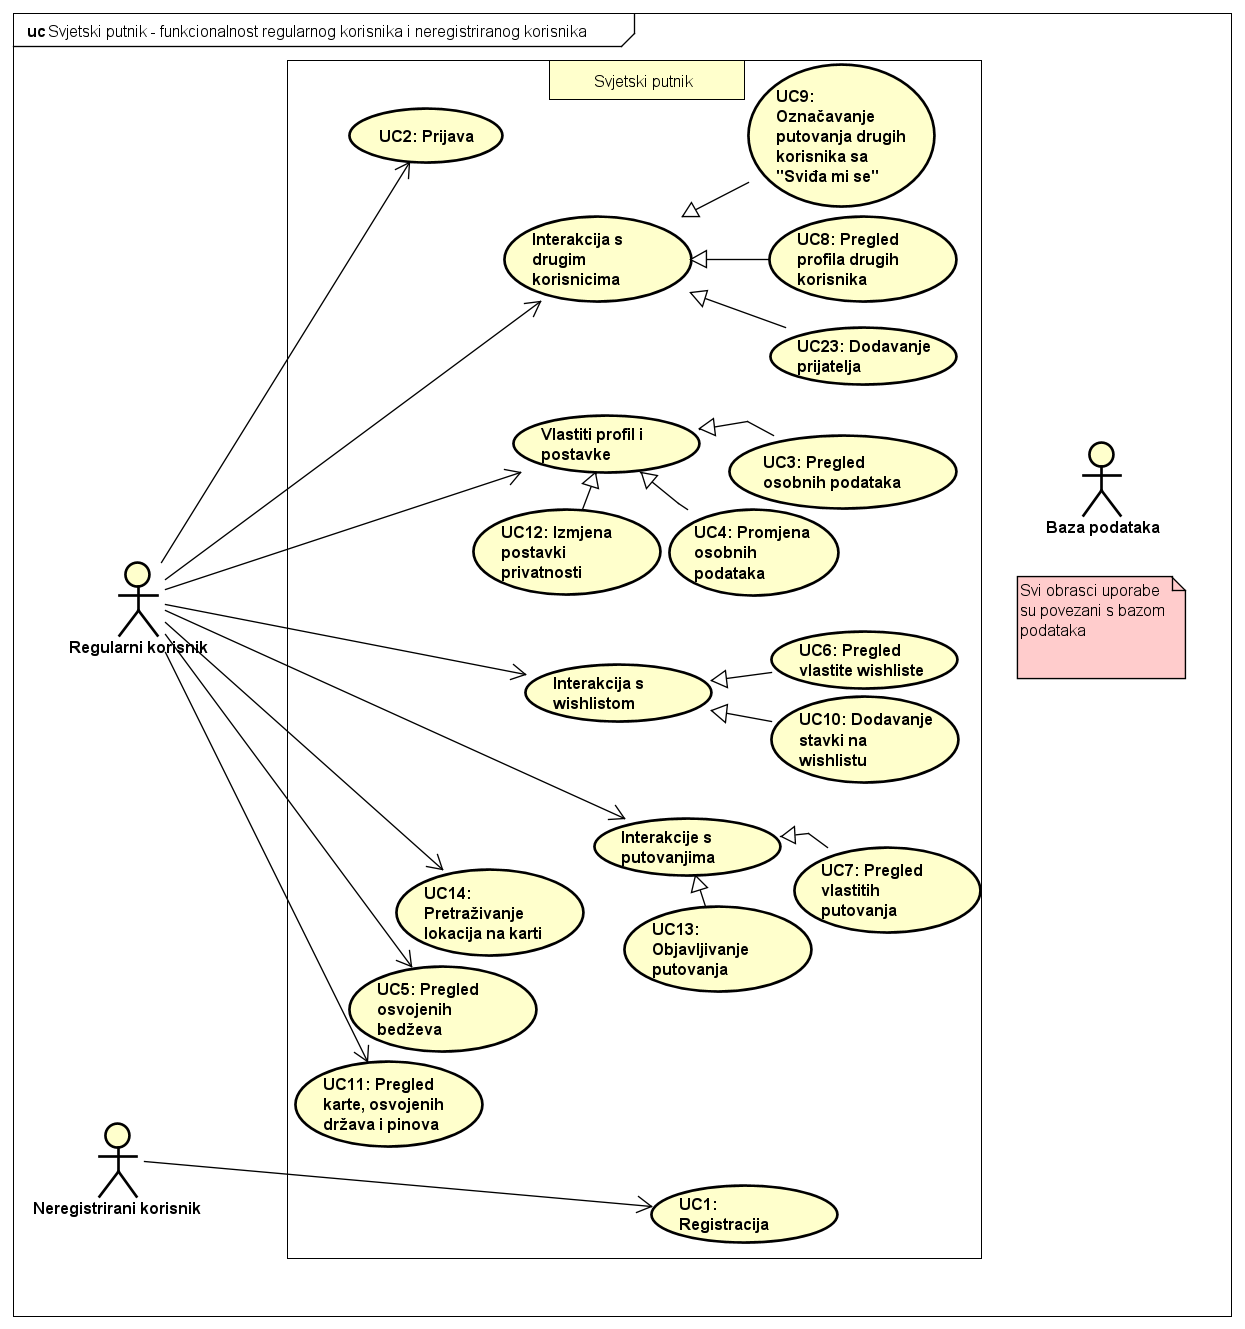
\includegraphics[scale=0.4]{slike/UC-regularnikorisnik-alt.png} %veličina slike u odnosu na originalnu datoteku i pozicija slike
                			\centering
                			\caption{UML dijagram obrazaca uporabe - regularni korisnik}
                			
                		\end{figure}
                		
                		\begin{figure}[H]
                			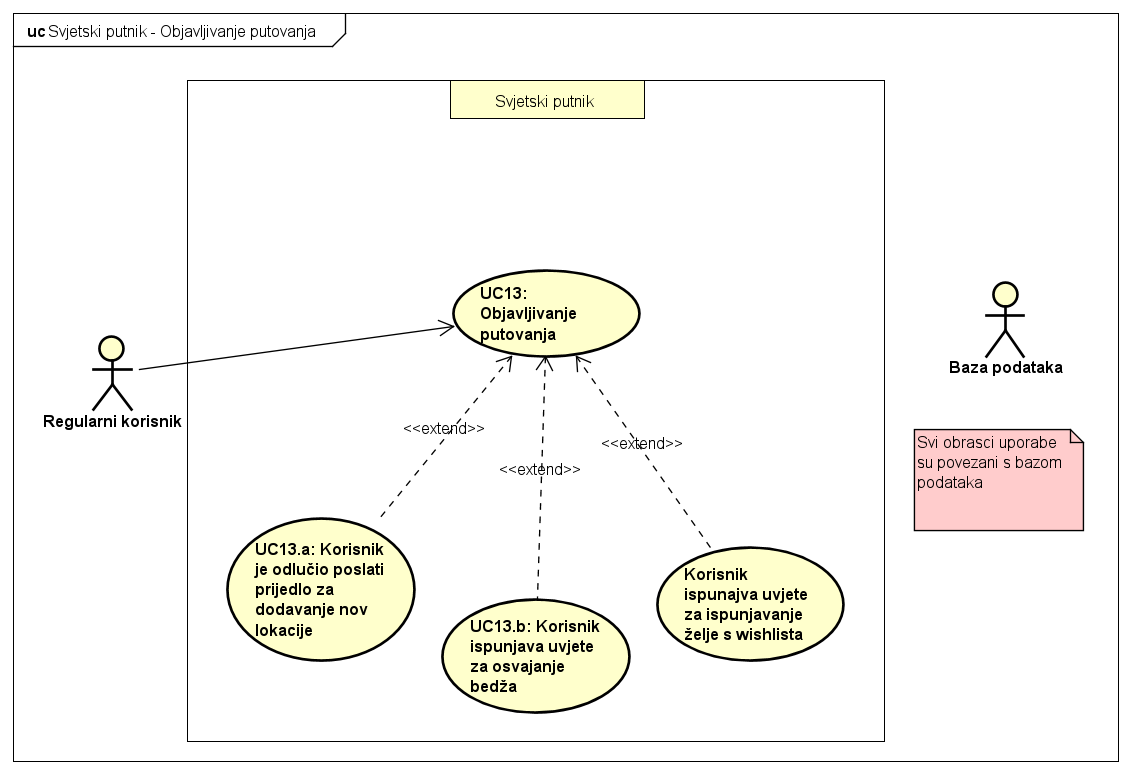
\includegraphics[scale=0.4]{slike/UC-objavljivanjeputovanja.png} %veličina slike u odnosu na originalnu datoteku i pozicija slike
                			\centering
                			\caption{UML dijagram obrazaca uporabe - objavljivanje putovanja}
                			
                		\end{figure}
        			
        				\begin{figure}[H]
                			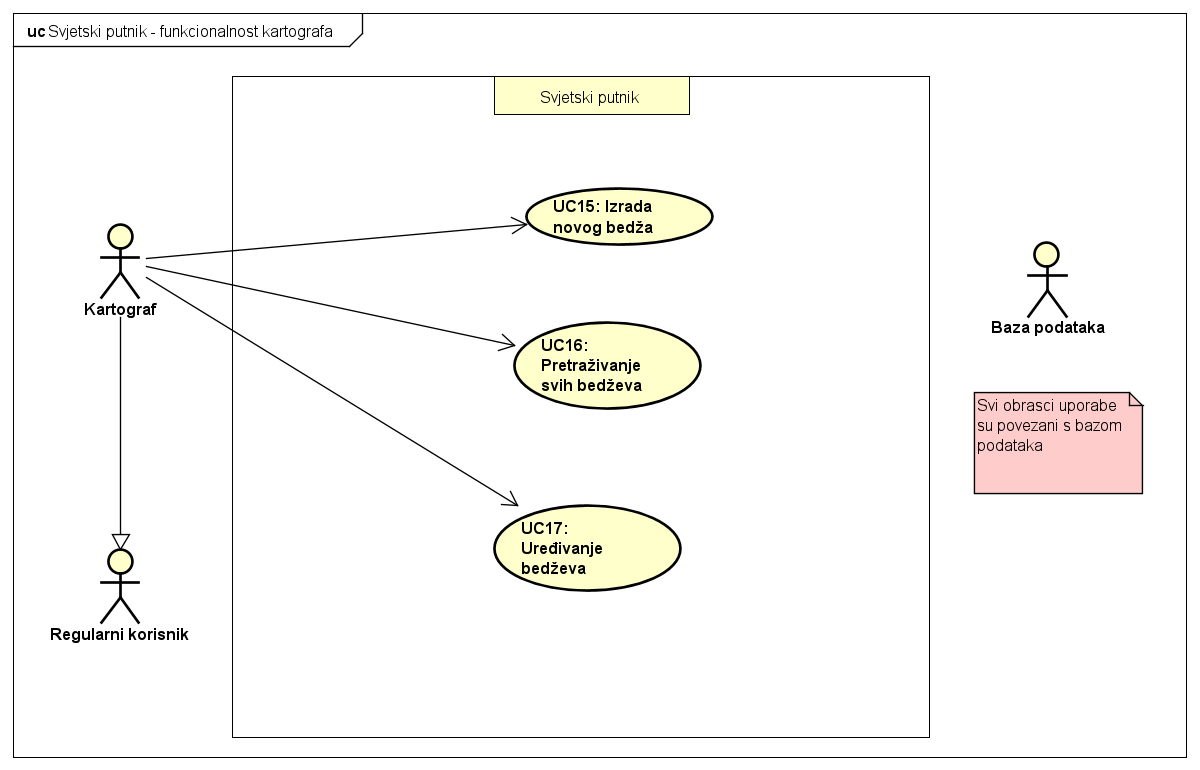
\includegraphics[scale=0.4]{slike/UC-kartograf.png} %veličina slike u odnosu na originalnu datoteku i pozicija slike
                			\centering
                			\caption{UML dijagram obrazaca uporabe - kartograf}
                			
                		\end{figure}
        			
        				\begin{figure}[H]
                			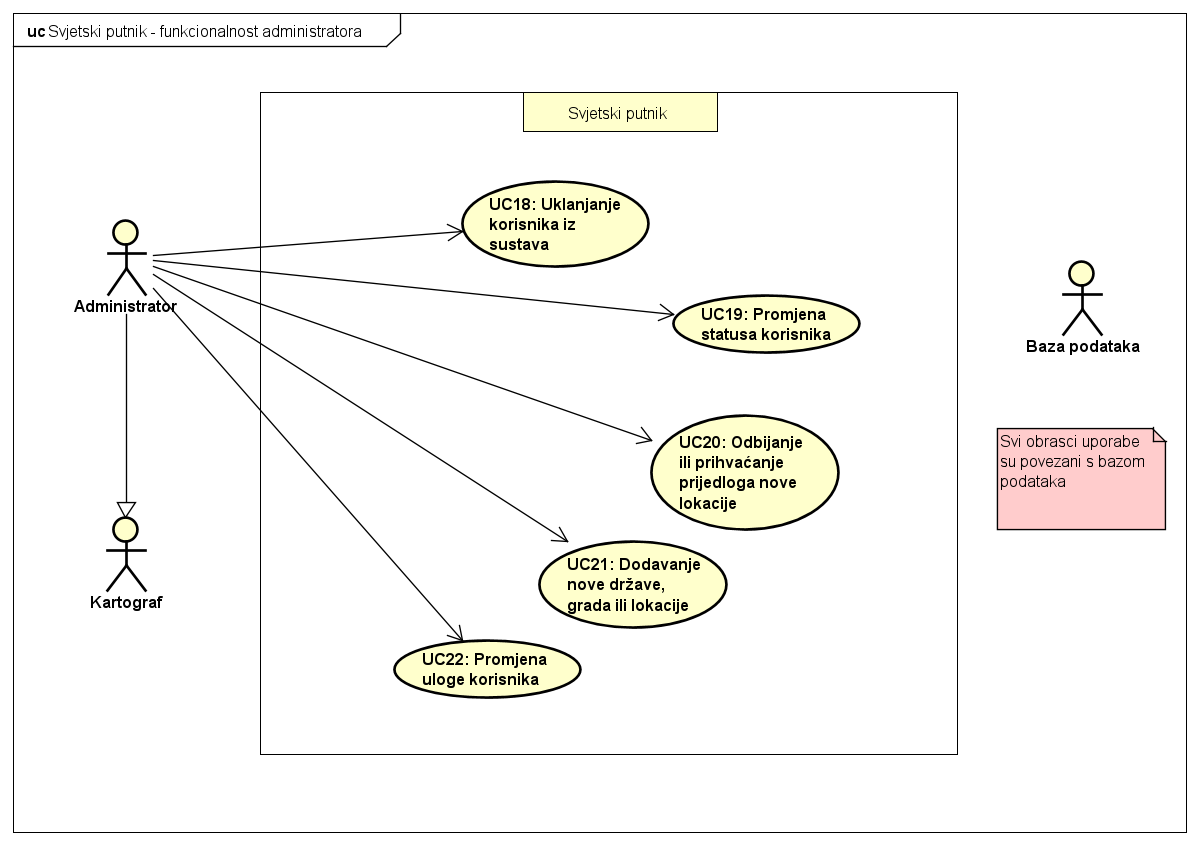
\includegraphics[scale=0.4]{slike/UC-dministrator.png} %veličina slike u odnosu na originalnu datoteku i pozicija slike
                			\centering
                			\caption{UML dijagram obrazaca uporabe - administrator}
                			
                		\end{figure}
				\eject		
				
			\subsection{Sekvencijski dijagrami}
			
			
			    Kartograf pristupa stranici "Bedževi", aplikacija prikazuje navedenu stranicu, Kartograf odabire "Novi Bedž", aplikacija prikazuje formu za kreiranje bedža. Kartograf ispunjava formu i šalje ispunjenu formu, aplikacija dodaje bedž u bazu podataka i kartografu prikazuje stranicu "Bedževi" (s vidljivim novim bedžem).
				\begin{figure}[H]
                	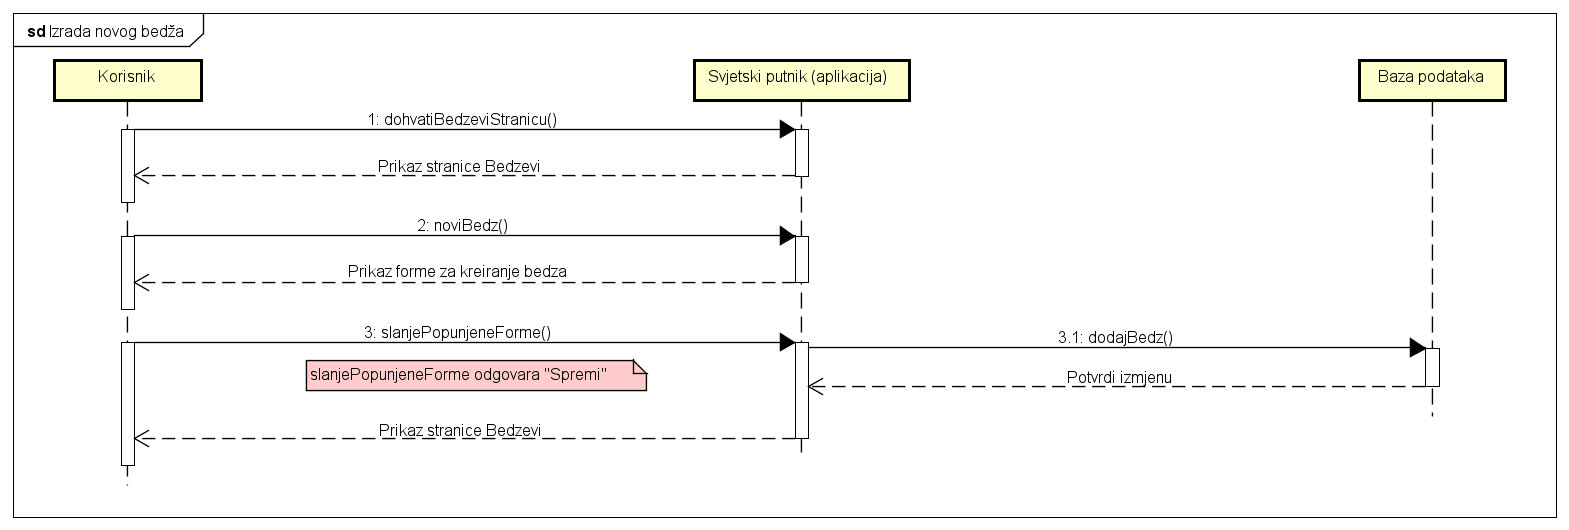
\includegraphics[scale=0.4]{slike/SD-izradabedza.png} %veličina slike u odnosu na originalnu datoteku i pozicija slike
                	\centering
                	\caption{UML sekvencijski dijagram - Izrada novog bedža}
                			
                \end{figure}
                
                
                Korisnik pristupa naslovnoj stranici, aplikacija dohvaća putovanja korisnika iz baze podataka te boja države i postavlja pinove na kartu. Aplikacija korisniku prikazuje naslovnicu sa obojenom kartom i pinovima.
                \begin{figure}[H]
                	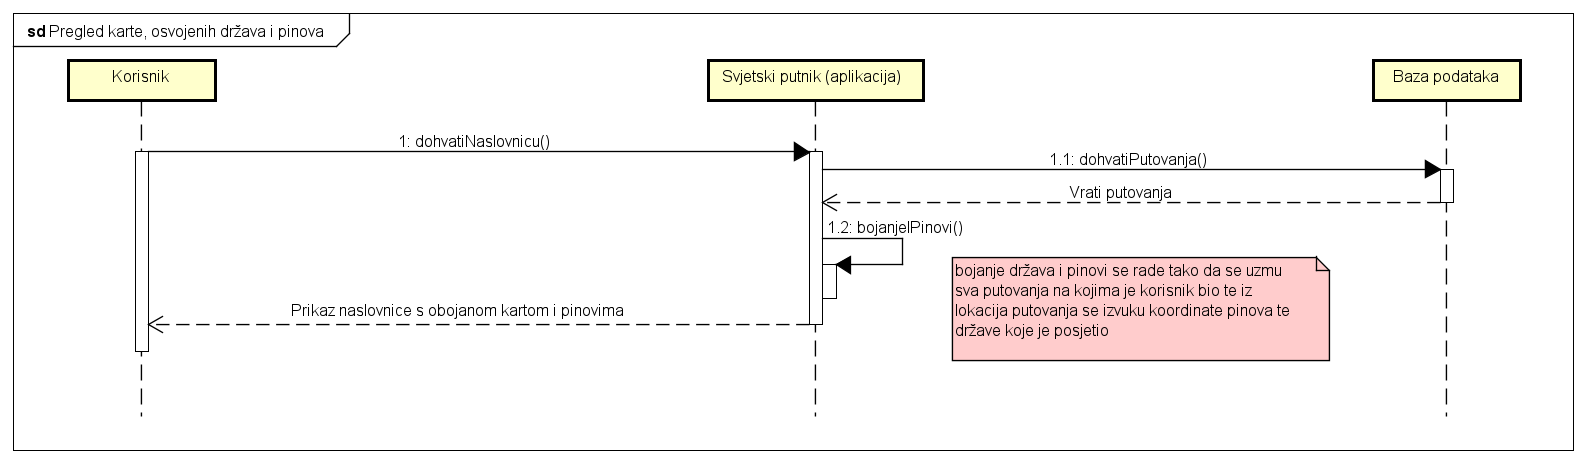
\includegraphics[scale=0.4]{slike/SD-pregledkarte.png} %veličina slike u odnosu na originalnu datoteku i pozicija slike
                	\centering
                	\caption{UML sekvencijski dijagram - Pregled karte, osvojenih država i pinova}
                			
                \end{figure}
                
                
                Korisnik odabire opciju "Nova objava", aplikacija korisniku prikazuje formu za izradu nove objave. Korisnik zatraži prikaz karte, aplikacija iz baze podataka dohvaća lokacije te prikazuje korisniku kartu s lokacijama. Korisnik ispunjava formu i označuje lokaciju. Korisnik šalje formu aplikaciji, aplikacija provjerava formu i ako lokacija ne postoji u bazi podataka sprema lokaciju (s flagom is\_suggestion). Aplikacija u bazu podataka sprema putovanje. Aplikacija dohvaća trenutne bedževe korisnika iz baze podataka i provjerava je li korisnik ispunio sva pravila za bilo koji bedž, ako je u bazi podataka se sprema osvojen bedž i uklanja trenutni bedž. Aplikacija dohvaća trenutnu wishlistu korisnika iz baze podataka i provjerava je li korisnik ispunjava uvjete bilo koje wishlist stavke, ako ispunjava u bazi podataka se sprema osvojen bedž i uklanja trenutni bedž. Aplikacija ponovno prikazuje stranicu bez forme s novim putovanjem dodanim.
                \begin{figure}[H]
                	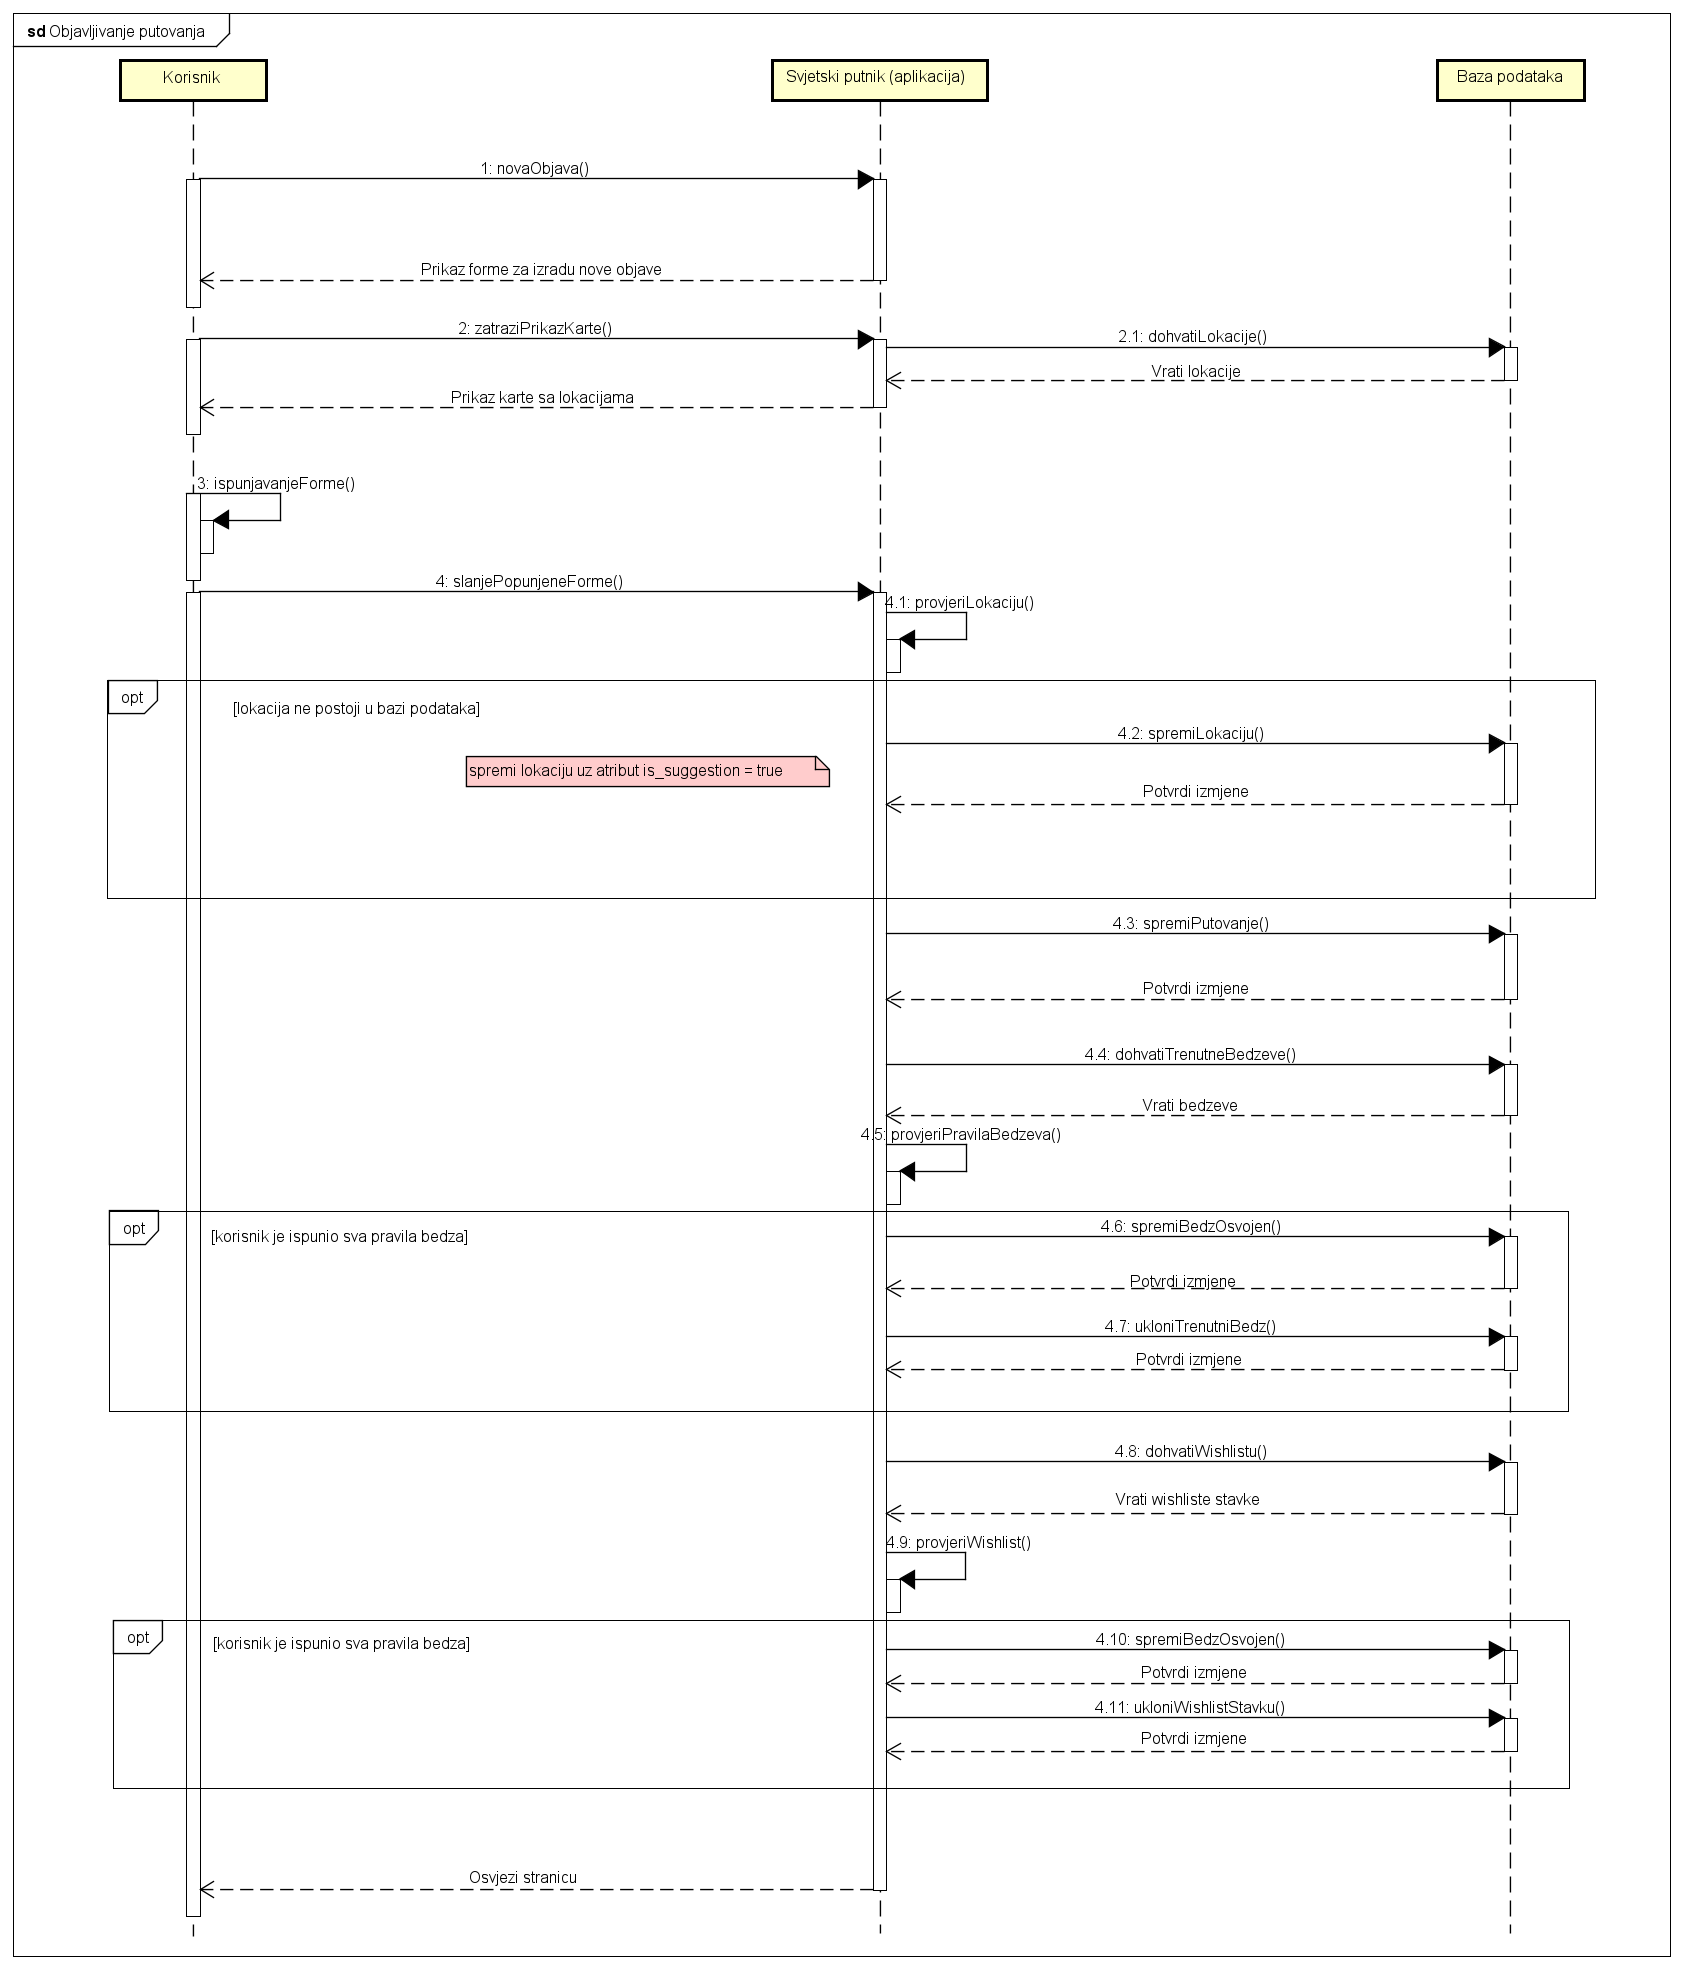
\includegraphics[scale=0.4]{slike/SD-objavljivanjeputovanja.png} %veličina slike u odnosu na originalnu datoteku i pozicija slike
                	\centering
                	\caption{UML sekvencijski dijagram - Objavljivanje putovanja}
                			
                \end{figure}
                
                
                Administrator odabire "Preporuke/prijedlozi (lokacija)", aplikacija dohvaća lokacije iz baze podataka, odabire one s flagom is\_suggestion i prikazuje ih Administratoru. Ako administrator smatra da je lokacija prihvatljiva onda prihvaća prijedlog te aplikacija ažurira u bazi podataka da je to prava lokacija, aplikacija prikazuje stranicu "Preporuke/prijedlozi (lokacija)". Ako administrator smatra da lokacije nije prihvatljiva onda odbija prijedlog te aplikacija uklanja lokaciju iz baze podataka te aplikacija prikazuje stranicu "Preporuke/prijedlozi (lokacija)".
                \begin{figure}[H]
                	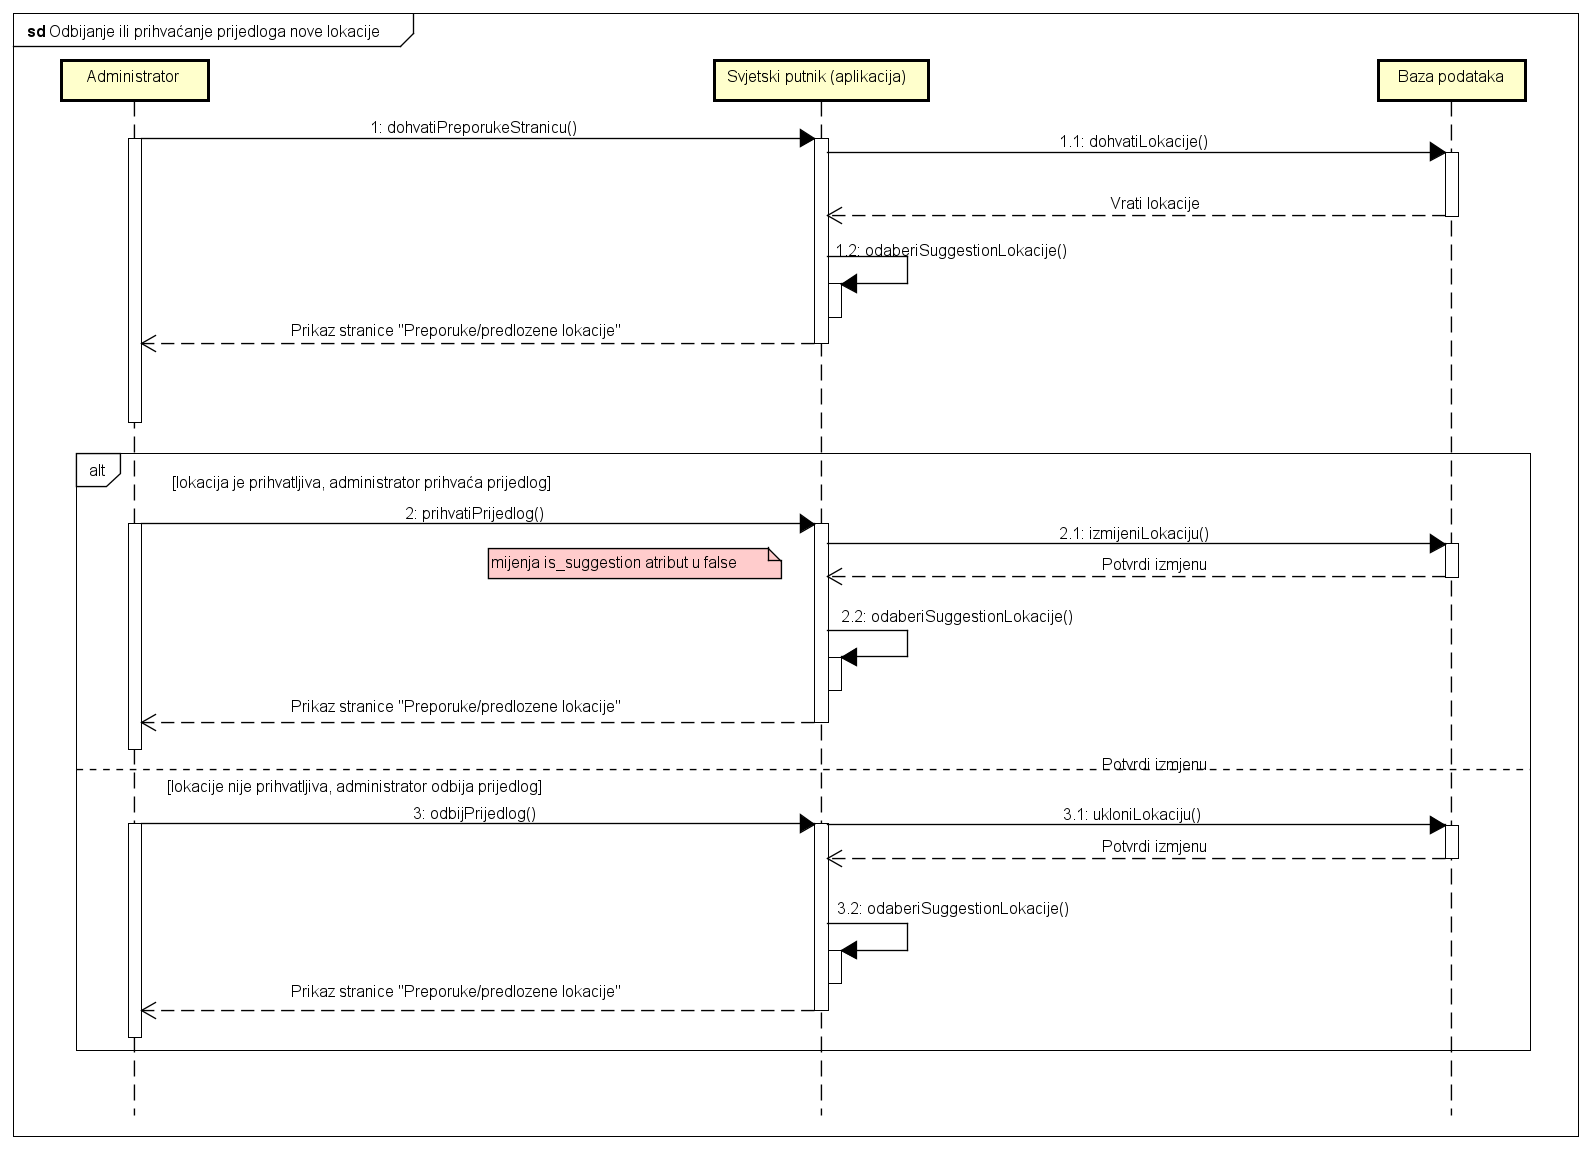
\includegraphics[scale=0.4]{slike/SD-odbijanjeprihvacanje.png} %veličina slike u odnosu na originalnu datoteku i pozicija slike
                	\centering
                	\caption{UML sekvencijski dijagram - Odbijanje ili prihvaćanje prijedloga nove lokacije}
                			
                \end{figure}
                
				
				\eject
	
		\section{Ostali zahtjevi}
		
		    
			\begin{packed_item}
			    \item Sustav treba omogućiti rad više korisnika u stvarnom vremenu
			    \item Neispravno korištenje korisničkog sučelja ne smije naručiti funkcionalnost sustava
			    \item Sustav mora biti jednostavan za korištenje
			    \item Veza prema bazi podataka treba biti zaštićena i brza
			    \item Korisničko sučelje mora podržavati hrvatsku abecedu pri unosu i prikazu tekstualnog sadržaja
			\end{packed_item}
			 
			 
			 
	